\documentclass[12pt,a4paper]{article}
\usepackage[utf8]{inputenc}
\usepackage[T1]{fontenc}
\usepackage{fontspec}
\usepackage[polish]{babel}
\usepackage{amsmath}
\usepackage{graphicx}
\usepackage[table,xcdraw]{xcolor}
\usepackage{hhline}
\usepackage{placeins}
\usepackage[margin=0.6in]{geometry}
\usepackage{appendix}
\usepackage{colortbl}
\usepackage{physics}
\usepackage{float}
\usepackage{datetime}
\usepackage{hyperref}

\title{Praca Domowa Termodynamika i Fizyka Statystyczna R 2021/2022}
\author{Kacper Cybiński}
% \newdate{date}{28}{01}{2022}
% \date{\displaydate{date}}
\date{\today}
\setlength\parindent{0pt}

\newcommand{\com}[1]{{\color{red} #1}}

\newcommand{\link}[2]{{\color{cyan} \href{#1}{#2}}}

\renewcommand{\emph}{\textbf}

\begin{document}

\maketitle

\section{Zadanie 1}

\begin{figure}[h!]
    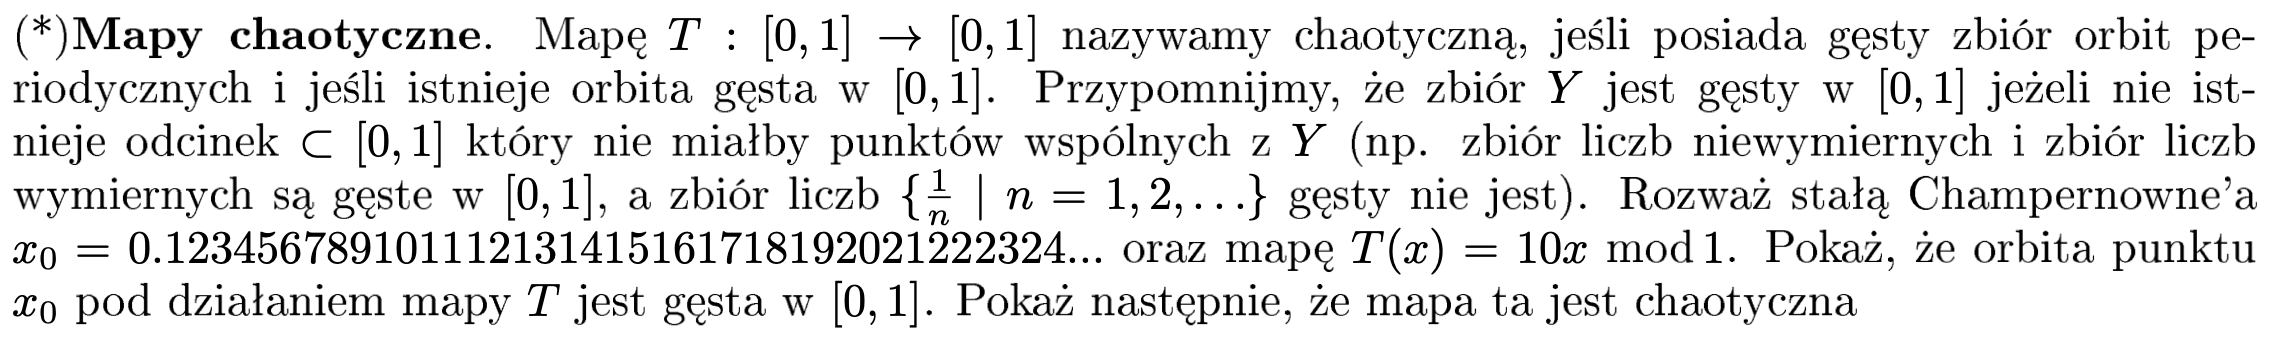
\includegraphics[width=\linewidth]{Zrzut ekranu 2022-05-19 o 08.10.03.png}
\end{figure}

\FloatBarrier

\section{Rozwiązanie}

Rozwiązanie jest poprzez machanie rękami, chętnie się dowiem jak poprawnie ściśle się to udowadnia. Niemniej, podzielmy sobie argumentację na dwie części, za gęstością orbity $x_0$ w $\qty[0,1]$ i za gęstością orbit w $\qty[0,1]$.

\subsection{Uzasadnienie gęstości orbity $x_0$ w $\qty[0,1]$}


Zauważamy, że stała Champernowne'a $x_{0}=0,12345678910111 \ldots$ jest skonstruowana poprzez zapisywania jako kolejnych liczb w rozwinięciu dziesiętnym poprzez kolejne liczby naturalne. 

Jak działa mapa T? Możemy myśleć o kolejnych działaniach mapy jako "przesunięcie"przecinka o jedno miejsce w prawo oraz usunięcie liczby jedności. Rozważmy dowolny punkt $y \in[0,1]$ oraz epsilonową kulę w której siedzi, $d(x, \epsilon)$. 

Orbita punktu $x_{0}$ jest gęsta w [0,1], jeśli dla dowolnego punktu $y\in\qty[0,1]$, w jego najbliższym otoczeniu znajdzie się element orbity $\mathrm{x}_{0}$. 

Jako, że stałą Champernowne'a konstruuje się dostawiając kolejne liczy naturalne do rozwinięcia dziesiętnego, po pewnej iteracji $T^{n}\left(x_{0}\right)$ otrzymamy liczbę postaci 
$$0, \mathrm{y} \, (0)_{k} \, a$$
gdzie a jest pewnym ciągiem liczby złożonym z kolejnych liczb naturalnych, tak jak wynika z konstrukcji liczby Champernowne'a. 

Jako że stała ta jest konstruowana poprzez dodawanie nieskończonej ilości liczb naturalnych, dla dowolnego $\epsilon$ możemy wybrać takie k, że 
$$T^{n}\left(x_{0}\right)-y<\epsilon$$. 
Możemy również z drugiej strony, wybrać taką iterację mapy $\mathrm{T}$, że $T^{n}\left(x_{0}\right)$ będzie postaci 
$$0,(y-1)\,(9)_{k} \,a$$ 
gdzie a znów jest ciągiem liczb naturalnych. Jako że do konstrukcji liczby Champernowne'a używamy nieskończonej ilości liczb naturalnych znajdziemy takie $\mathrm{k}$ dla którego $$y-T^{n}\left(x_{0}\right)<\epsilon$$. 
Jako że dla każdej liczby z $[0,1]$ możemy przeprowadzić takie rozumowanie, dochodzimy do wniosku, że \emph{orbita $\mathrm{x}_{0}$ jest gęsta $\mathrm{w}[0,1]$}.

\subsection{Uzasadnienie, że zbiór orbit periodycznych jest gęsty w $\qty[0,1]$}

Jedyne punkty mające orbity periodyczne mapy T mają postać liczb okresowych np $0,(1234)=0,123412341234 \ldots$ Chcemy teraz pokazać, że dla dowolnego punktu $y \in[0,1]$ nie potrafimy wybrać takiego otoczenia $d(y, \epsilon)$ do którego nie należałby punkt ze zbioru orbit mapy T. 

Oznaczmy ilość cyfr w rozwinięciu dziesiętnym liczby $y$ jako $m$. skonstruujmy najpierw punkt $x$, który ma orbitę periodyczną, gdzie $x>y$ oraz $x-y<\epsilon$. Niech $x$ ma postać 
$$x=0,\left(10^{m} y(0)_{k} 1\right)$$
czyli $x=10^{m} y 000 . .(k-$ razy ... $) 001 y 00 \ldots$ zapiszmy tą liczbę jako ułamek, oraz przejdźmy z $\mathrm{k}$ do nieskończoności.\\
Będziemy chcieli pokazać, że jesteśmy w stanie zbliżyć się dowolnie blisko od dołu i od góry do dowolnej liczby, co będzie oznaczało, że jesteśmy w stanie pokryć cały odcinek $\qty[0,1]$ tymi orbitami.
$$
\begin{gathered}
0,\left(\left(10^{m} y\right)(0)_{k} 1\right)=x \\
\left(10^{m} y\right)(0)_{k} 1,\left(\left(10^{m} y\right)(0)_{k} 1\right)=10^{m+k+1} x \\
\left(10^{m} y\right)(0)_{k} 1=x\left(10^{m+k+1}-1\right) \\
x=\frac{\left(10^{m} y\right)(0)_{k} 1}{\left(10^{m+k+1}-1\right)} \\
x=\frac{\left(10^{m} y\right) \cdot 10^{k+1}+1}{10^{m+k+1}-1} \\
\lim _{k \rightarrow \infty} x=\frac{\left(10^{m} y\right)}{10^{m}}=y
\end{gathered}
$$
Możemy przeprowadzić podobne rozumowanie z liczbą $x<y$, która ma postać $x=0,\left(\left(10^{m} y-1\right)(9)_{k}\right)$ czyli
$$
x=0,\left(10^{m} y-1\right) 99(k-r a z y) 99\left(10^{m} y-1\right) 99 \ldots
$$
$$
\begin{gathered}
0,\left(\left(10^{m} y-1\right)(9)_{k}\right)=x \\
\left(10^{m} y-1\right)(9)_{k},\left(\left(10^{m} y-1\right)(9)_{k}\right)=10^{m+k} x \\
\left(10^{m} y-1\right)(9)_{k}=x\left(10^{m+k}-1\right) \\
x=\frac{\left(10^{m} y-1\right)(9)_{k}}{\left(10^{m+k}-1\right)} \\
x=\frac{\left(10^{m} y\right) \cdot 10^{k}-1}{10^{m+k}-1} \\
\lim _{k \rightarrow \infty} x=\frac{\left(10^{m} y\right)}{10^{m}}=y
\end{gathered}
$$
W związku z tym widzimy, że dla dowolnej liczby wymiernej należącej do zbioru $[0,1]$, dla dowolnego jej otoczenia będziemy mieć punkty należące do zbioru orbit periodycznych, czyli jest to zbiór gęsty. 

Pokazaliśmy więc że mapa ma gęsty zbiór orbit periodycznych oraz istnieje orbita gęsta w $[0,1]$ czyli \emph{mapa $\mathrm{T}$ jest chaotyczna}, co należało dowieść.

\end{document}